\documentclass{article}
\usepackage{graphicx}
\usepackage{amsmath, amssymb, amsthm}
\usepackage{booktabs}
\usepackage{hyperref}

\theoremstyle{definition}
\newtheorem{definition}{Definition}
\newtheorem{theorem}{Theorem}
\newtheorem{lemma}{Lemma}

\newcommand{\pre}{\mathit{pre}}
\newcommand{\pref}{\mathit{pre}^f}
\newcommand{\prew}{\mathit{pre}^w}
\newcommand{\preg}{\mathit{pre}^g}
\newcommand{\add}{\mathit{add}}
\newcommand{\del}{\mathit{del}}
\newcommand{\num}{\mathit{num}}
\newcommand{\eff}{\mathit{eff}}
\newcommand{\fail}{\mathit{fail}}
\newcommand{\act}{\mathit{act}}
\newcommand{\fin}{\mathit{fin}}
\newcommand{\cf}{\mathit{cf}}
\newcommand{\wt}{\mathit{wt}}

\title{Social Laws in Multi-Agent Planning:\\A Survey of Compilation-Based Verification}
\author{Evgeny Mishlyakov}
\date{March 2026}

\begin{document}

\maketitle

\begin{abstract}
A \emph{social law} is a restriction on a multi-agent planning system designed to prevent inter-agent conflicts while preserving each agent's ability to achieve its goal independently. The central property of interest is \emph{robustness}: a social law is robust if every combination of individually valid agent plans can be jointly executed under any adversarial scheduling without deadlock, action failure, or goal violation.

This survey covers three compilation-based methods for verifying robustness. Karpas et al.\ introduced the reduction to classical planning via an $(n+1)$-copy state encoding, but the original formulation contains a flaw in deadlock detection. Nir et al.\ extended and corrected this approach to the numeric setting (MA-SNP), handling numeric fluents and wait-for conditions over numeric constraints. Tuisov et al.\ generalized further to arbitrary instantaneous-action formalisms with first-order-logic preconditions, using an explicit two-stage execution model.

We present a unified implementation of the numeric and general compilations within the Unified Planning Framework (UPF), together with an automatic translation from restricted-task representations to numeric STRIPS. We evaluate both verifiers on a completed run and report aggregate results on 322 benchmark configurations (644 verifier/configuration pairs). The resulting picture is mixed rather than one-sided: the simple compilation finds easy\\
 counterexamples quickly and is especially strong on \texttt{numeric\_grid}, while the general compilation proves robustness more often and performs better on domains such as \texttt{driverlog}, \texttt{zenotravel}, and \texttt{numeric\_markettrader}. The run also exposes benchmark-specific failure modes, most notably worker failures on \texttt{intersection} and internal errors on \texttt{numeric\_expedition}.
\end{abstract}

% ============================================================
\section{Introduction}
% ============================================================

In a multi-agent planning system, independently acting agents share an environment. Because each agent plans for itself in isolation, their plans may interact destructively: one agent's action may delete a precondition required by another, or two agents may enter a livelock waiting indefinitely for one another.

One principled approach to avoiding such interactions is the \emph{social law} (SL) paradigm~\cite{tennenholtz1989}. A social law modifies the planning problem available to each agent---removing actions, tightening preconditions, or annotating certain preconditions as \emph{wait-for}---so that conflicts are structurally prevented. A law that succeeds is called \emph{robust}: no matter what individually valid plan each agent chooses, and no matter how an adversarial scheduler interleaves their execution, every agent achieves its goal.

Verifying robustness by direct enumeration is infeasible. Karpas et al.~\cite{karpas2017} proposed reducing it to classical planning: construct a single-agent planning task $\Pi'$ whose solutions correspond \emph{exactly} to counterexamples to robustness. Robustness then holds iff $\Pi'$ is unsolvable---and unsolvability can be certified by a planner.

Two follow-up lines extend this approach. Nir et al.~\cite{nir2023} lift the compilation to the \emph{numeric} setting, supporting numeric fluents and wait-for conditions over numeric constraints, and simultaneously fix a bug in the original deadlock-detection logic. Tuisov et al.~\cite{tuisov2025} provide a fully general compilation that is parametric in the action formalism, requiring only that preconditions be computable boolean formulas; this subsumes both classical and numeric STRIPS as special cases.

% ============================================================
\section{Background}
% ============================================================

\subsection{Multi-Agent Planning Formalisms}

\paragraph{MA-STRIPS.}
A \emph{multi-agent STRIPS task}~\cite{brafman2008} is a tuple
\[
  \Pi = \langle F,\, \{A_i\}_{i=1}^n,\, I,\, \{G_i\}_{i=1}^n \rangle,
\]
where $F$ is a finite set of Boolean facts, $I \subseteq F$ is the initial state, and for each agent $i \in [n] := \{1,\ldots,n\}$: $A_i$ is agent $i$'s action set and $G_i \subseteq F$ is its goal. Each action $a \in A_i$ is a triple $(\pre(a), \add(a), \del(a))$ with $\pre(a), \add(a), \del(a) \subseteq F$. Applying $a$ in state $s$ (when $\pre(a) \subseteq s$) yields $(s \setminus \del(a)) \cup \add(a)$. The \emph{individual projection} of $\Pi$ onto agent $i$ is $\Pi_i = \langle F, A_i, I, G_i \rangle$.

\paragraph{Multi-Agent Simple Numeric Planning (MA-SNP).}
Nir et al.~\cite{nir2023} extend MA-STRIPS to the \emph{numeric restricted task} (RT) formalism of Hoffmann~\cite{hoffmann2003}. A \emph{multi-agent restricted task} (MART) is
\[
  \Pi = \langle P,\, V,\, s_0,\, \{A_i\}_{i=1}^n,\, \{G_i\}_{i=1}^n \rangle,
\]
where $P$ is a set of propositional variables, $V$ is a set of numeric variables, and $s_0 = \langle s_0^p, s_0^n \rangle$ is the initial state with $s_0^p \subseteq P$ and $s_0^n$ a full numeric assignment. Each action $a \in A_i$ has:
\begin{itemize}
  \item propositional preconditions $\mathit{pre}_p(a) \subseteq P$,
  \item numeric preconditions $\mathit{pre}_n(a)$: a set of constraints of the form $v \geq w_0$ with $v \in V$, $w_0 \in \mathbb{Q}$,
  \item propositional effects $\add(a), \del(a) \subseteq P$,
  \item numeric effects $\num(a)$: a set of updates $v \mathrel{+}= k_v$ with $k_v \neq 0$.
\end{itemize}
The full precondition is $\pre(a) = \mathit{pre}_p(a) \cup \mathit{pre}_n(a)$.

\paragraph{General Formalism.}
Tuisov et al.~\cite{tuisov2025} work with a fully general formalism:
\[
  \Pi = \langle V,\, \{A_i\}_{i=1}^n,\, I,\, \{G_i\}_{i=1}^n \rangle,
\]
where $V$ is a set of variables with arbitrary domains (Boolean, finite-domain, or numeric), and $\pre(a)$ is a \emph{computable Boolean formula} over $V$. The result of applying $a$ to state $s$ is denoted $s[a]$.

\subsection{Social Laws and Wait-For Preconditions}

\begin{definition}[Social Law]
A \emph{social law} $l$ is a function that maps a multi-agent task $\Pi$ to a modified task $\Pi^l$. Such modifications may include removing actions, strengthening preconditions, adding auxiliary facts, and annotating preconditions as \emph{wait-for}.
\end{definition}

\paragraph{Wait-for semantics.}
For each action $a$, its preconditions are partitioned into:
\begin{itemize}
  \item $\pref(a)$: \emph{failure preconditions}---if violated during execution, the action fails immediately.
  \item $\prew(a)$: \emph{wait-for preconditions}---if violated, the agent blocks until they are satisfied.
\end{itemize}
The scheduler may only execute action $a$ for agent $i$ when $\prew(a)$ holds in the current global state.

\subsection{Execution Model}

Let $\pi^{jnt} = \{\pi_i\}_{i=1}^n$ be a set of individual plans. An execution state is a pair $\langle s, \mathbf{j} \rangle$ where $s$ is the current world state and $\mathbf{j} = (j_1, \ldots, j_n)$ records each agent's position in its plan.

At each step, the scheduler selects an agent $i$ such that $\prew(\pi_i[j_i])$ holds in $s$. Four terminal outcomes are possible:

\begin{enumerate}
  \item[\textbf{(S)}] \textbf{Success}: all agents finish; $s \models \bigwedge_{i=1}^n G_i$.
  \item[\textbf{(F)}] \textbf{Action Failure}: an agent executes $a$ with $s \not\models \pref(a)$.
  \item[\textbf{(D)}] \textbf{Deadlock}: no agent can act ($\prew$ of every pending action is unsatisfied), but some agent is not done.
  \item[\textbf{(G)}] \textbf{Goal Miss}: all agents finish; $s \not\models G_i$ for some $i$.
\end{enumerate}

Outcomes (F), (D), (G) are collectively \emph{failures}. Let $R^{jnt}(\Pi)$ denote the set of maximal joint executions of $\Pi$, and $R^{jnt}_*(\Pi) \subseteq R^{jnt}(\Pi)$ the successful ones.

\begin{definition}[Robustness~\cite{nir2023}]
A multi-agent task $\Pi$ has a \emph{robust} social law iff $R^{jnt}_*(\Pi) \neq \emptyset$ and $R^{jnt}_*(\Pi) = R^{jnt}(\Pi)$.
\end{definition}

Equivalently: the social law $l$ applied to $\Pi$ is robust iff every set of individually valid plans jointly succeeds under every possible scheduling.

% ============================================================
\section{The Original Compilation (Karpas et al., 2017)}
% ============================================================

\subsection{Construction}

Given $\Pi^l = \langle F, \{A_i\}_{i=1}^n, I, \{G_i\}_{i=1}^n \rangle$, Karpas et al.\ construct a classical planning task
\[
  \Pi' = \langle F', A', I', G' \rangle
\]
as follows.

\paragraph{Facts.}
\[
  F' = \underbrace{\{f_i \mid f \in F,\ i \in [n]\}}_{\text{local copies}}
  \;\cup\; \underbrace{\{f_g \mid f \in F\}}_{\text{global copy}}
  \;\cup\; \underbrace{\{\mathit{wt}_{f,i} \mid f \in F,\ i \in [n]\}}_{\text{waiting flags}}
  \;\cup\; \{\mathit{fin}_i \mid i \in [n]\}
  \;\cup\; \{\mathit{failure},\, \act\}.
\]

\paragraph{Initial state and goal.}
\[
  I' = \{\act\} \cup \{f_i \mid f \in I,\ i \in [n]\} \cup \{f_g \mid f \in I\}.
\]
\[
  G' = \{\mathit{failure}\} \cup \{f^c \mid f \in F\} \cup \{\mathit{fin}_i \mid i \in [n]\}.
\]

\paragraph{Action variants.}
For each $a \in A_i$, three variants are introduced; all apply the effects of $a$ to the local copy $i$, but differ in their treatment of the global copy.

\medskip
\noindent\textbf{Success action $a_i^s$}: $a$ succeeds jointly.
\begin{align*}
  \pre(a_i^s) &= \act \;\wedge \textstyle\bigwedge_{f \in \pre(a)} (f_i \wedge f_g), \\
  \add(a_i^s) &= \{f_i, f_g \mid f \in \add(a)\}, \quad
  \del(a_i^s) = \{f_i, f_g \mid f \in \del(a)\}.
\end{align*}

\medskip
\noindent\textbf{Failure action $a_i^f$}: a non-wait-for precondition of $a$ fails in the global state.
\begin{align*}
  \pre(a_i^f) &= \act \;\wedge \textstyle\bigwedge_{f \in \pre(a)} f_i \;\wedge \bigwedge_{f \in \prew(a)} f_g \;\wedge \bigvee_{f \in \pref(a)} \neg f_g, \\
  \add(a_i^f) &= \{\mathit{failure}\} \cup \{f_i \mid f \in \add(a)\}, \quad
  \del(a_i^f) = \{f_i \mid f \in \del(a)\}.
\end{align*}

\medskip
\noindent\textbf{Wait/deadlock action $a_i^{w,x}$} for each $x \in \prew(a)$: $a$'s wait-for precondition $x$ fails in the global state.
\begin{align*}
  \pre(a_i^{w,x}) &= \act \;\wedge \textstyle\bigwedge_{f \in \pre(a)} f_i \;\wedge \neg x_g, \\
  \add(a_i^{w,x}) &= \{\mathit{failure},\, \mathit{wt}_{x,i}\} \cup \{f_i \mid f \in \add(a)\}, \quad
  \del(a_i^{w,x}) = \{f_i \mid f \in \del(a)\}.
\end{align*}

\paragraph{END actions.}
Two versions per agent: $\mathit{END}_i^s$ (goal met in both copies) and $\mathit{END}_i^f$ (goal met locally but not globally). Both delete $\act$, so no regular actions can fire afterward.

\paragraph{CHECK actions.}
For each $f \in F$, two post-termination actions verify deadlock genuineness:
$\mathit{CHECK\text{-}NO}\text{-}f$ asserts $\neg f_g$, and
$\mathit{CHECK\text{-}NO\text{-}WAITING}\text{-}f$ asserts $\bigwedge_i \neg \mathit{wt}_{f,i}$.
Both add $f^c$ (required for the goal). Together they enforce: if $\mathit{wt}_{f,i}$ is true at the end then $f$ does not hold in the global state.

\subsection{Correctness}

\begin{theorem}[Karpas et al., 2017]
  $\Pi'$ is solvable if and only if $\Pi^l$ is not rationally robust (assuming each $\Pi_i$ is individually solvable).
\end{theorem}

The key invariants are: (i) local copy $i$ faithfully tracks agent $i$'s individual execution; (ii) the global copy tracks the adversarially interleaved joint execution; (iii) the CHECK actions certify that waited-for facts remain false forever.

\subsection{Deficiency in Deadlock Detection}

As noted by Tuisov and Karpas~\cite{tuisov2020}, the original formulation contains a subtle error. The wait action $a_i^{w,x}$ fires as soon as $x_g$ is false, \emph{regardless of whether} $x$ could become true before agent $i$ next acts. The CHECK mechanism is supposed to retroactively verify that $x$ truly remains false, but the original encoding does not correctly prevent other agents from satisfying $x$ later under all schedules. This can cause the compilation to accept spurious deadlock witnesses, compromising soundness. The numeric compilation of Nir et al.\ corrects this by strengthening the success action $a_i^s$ to \emph{forbid} increasing a waited-for numeric variable past its threshold if some other agent is declared waiting for it.

% ============================================================
\section{Numeric Compilation (Nir et al., 2023)}
% ============================================================

\subsection{Construction}

Given a MART $\Pi = \langle P, V, s_0, \{A_i\}_{i=1}^n, \{G_i\}_{i=1}^n \rangle$, the compiled task $\widetilde{\Pi} = \langle \widetilde{P}, \widetilde{V}, \widetilde{A}, \widetilde{s}_0, \widetilde{G} \rangle$ maintains $n+1$ copies of each propositional and numeric variable.

\paragraph{Variables.}
Let $P_i = \{p_i \mid p \in P\}$ and $V_i = \{v_i \mid v \in V\}$ for $i \in [n] \cup \{g\}$. Waiting flags are:
\[
  Wt = \{\wt_i,\, \wt_\psi \mid \psi \in \prew(a),\, a \in A_i,\, i \in [n]\},
\]
where $\psi$ is either a propositional atom or a numeric constraint $v \geq w_0$. Control atoms are:
\[
  Bk = \{\act,\, \fail,\, \cf\} \cup \{\fin_i \mid i \in [n]\}.
\]
Thus $\widetilde{P} = Wt \cup Bk \cup \bigcup_{i \in [n] \cup \{g\}} P_i$ and $\widetilde{V} = \bigcup_{i \in [n] \cup \{g\}} V_i$.

\paragraph{Initial state and goal.}
\[
  \widetilde{s}_0^p = \{\act\} \cup \{p_i \mid p \in s_0^p,\ i \in [n] \cup \{g\}\}, \quad
  \widetilde{s}_0^n[v_i] = s_0^n[v] \text{ for all } v \in V,\ i \in [n] \cup \{g\}.
\]
\[
  \widetilde{G} = \{\fail\} \cup \{\fin_i \mid i \in [n]\}.
\]

\paragraph{Four action variants.}
For each $a \in A_i$, the compilation produces four versions.

\medskip
\noindent\textbf{(1) Success action $a_i^s$}: applicable when both local and global copies satisfy all preconditions, no agent is in deadlock waiting for a condition that $a$ would violate, and no action conflict has occurred.
\begin{align*}
  \pre(a_i^s) &= \act \wedge \neg \wt_i \wedge \neg \cf \\
    &\wedge \textstyle\bigwedge_{\psi \in \pre(a)} (\psi_i \wedge \psi_g)
     \wedge \textstyle\bigwedge_{p \in \add(a)} \neg \wt^p \\
    &\wedge \textstyle\bigwedge_{\substack{v \mathrel{+}= k_v \in \num(a) \\ w_0 \in W_v}} \!\!
       \bigl(\neg \wt^{v \geq w_0} \vee (v_g < w_0 - k_v)\bigr), \\
  \add(a_i^s) &= \{p_i, p_g \mid p \in \add(a)\}, \quad
  \del(a_i^s) = \{p_i, p_g \mid p \in \del(a)\}, \\
  \num(a_i^s) &= \{v_i \mathrel{+}= k,\, v_g \mathrel{+}= k \mid v \mathrel{+}= k \in \num(a)\}.
\end{align*}
Here $W_v = \{w_0 \mid v \geq w_0 \in \bigcup_{i'} (G_{i'} \cup \mathit{pre}_n(A_{i'}))\}$ is the set of relevant thresholds for variable $v$. The last precondition line encodes the key \textbf{deadlock-preservation invariant}: if some agent declared it is waiting for $v \geq w_0$, then no other agent may increase $v$ past $w_0$, preventing spurious satisfaction of the waited-for condition.

\medskip
\noindent\textbf{(2) Fail-action $a_i^f$}: a non-wait-for precondition of $a$ fails in the global copy.
\begin{align*}
  \pre(a_i^f) &= \act \wedge \neg \wt_i \wedge \neg \cf
    \wedge \textstyle\bigwedge_{\psi \in \pre(a)} \psi_i
    \wedge \textstyle\bigwedge_{\psi \in \prew(a)} \psi_g
    \wedge \textstyle\bigvee_{\psi \in \pref(a)} \neg \psi_g, \\
  \add(a_i^f) &= \{\fail, \cf\} \cup \{p_i \mid p \in \add(a)\}, \quad
  \del(a_i^f) = \{p_i \mid p \in \del(a)\}, \\
  \num(a_i^f) &= \{v_i \mathrel{+}= k \mid v \mathrel{+}= k \in \num(a)\}.
\end{align*}

\medskip
\noindent\textbf{(3) Deadlock action $a_i^{wt_\varphi}$} for each $\varphi \in \prew(a)$: the wait-for condition $\varphi$ is false in the global copy.
\begin{align*}
  \pre(a_i^{wt_\varphi}) &= \act \wedge \neg \wt_i \wedge \neg \cf
    \wedge \neg \varphi_g
    \wedge \textstyle\bigwedge_{\psi \in \pre(a)} \psi_i, \\
  \add(a_i^{wt_\varphi}) &= \{\wt_\varphi, \fail, \wt_i\} \cup \{p_i \mid p \in \add(a)\}, \quad
  \del(a_i^{wt_\varphi}) = \{p_i \mid p \in \del(a)\}, \\
  \num(a_i^{wt_\varphi}) &= \{v_i \mathrel{+}= k \mid \ldots\}.
\end{align*}
Setting $\wt_i$ permanently marks agent $i$ as waiting; no action can delete $\wt_i$. The deadlock-preservation invariant in $a_i^s$ ensures $\varphi_g$ can never later become true once $\wt_\varphi$ is set.

\medskip
\noindent\textbf{(4) Local action $a_i^l$}: applicable after a deadlock or action conflict; updates only the local copy.
\begin{align*}
  \pre(a_i^l) &= \act \wedge (\wt_i \vee \cf) \wedge \textstyle\bigwedge_{\psi \in \pre(a)} \psi_i, \\
  \add(a_i^l) &= \{p_i \mid p \in \add(a)\}, \quad
  \del(a_i^l) = \{p_i \mid p \in \del(a)\}, \quad
  \num(a_i^l) = \{v_i \mathrel{+}= k \mid v \mathrel{+}= k \in \num(a)\}.
\end{align*}
Local actions allow each agent to complete a valid individual plan in its local copy after failure, supplying the required $\fin_i$ atoms.

\paragraph{END actions.}
$\mathit{END}_i^s$: agent $i$ achieved $G_i$ in both copies (adds $\fin_i$, deletes $\act$).
$\mathit{END}_i^f$: agent $i$ achieved $G_i$ locally but not globally (additionally adds $\fail$).

\subsection{Correctness}

\begin{theorem}[Nir et al., 2023]
  $\widetilde{\Pi}$ is solvable $\Longleftrightarrow$ $\Pi$ is not robust.
\end{theorem}

The proof has three lemmas. (L1) Any plan $\pi'$ for $\widetilde{\Pi}$ projects to a valid individual plan $\pi_i$ for each agent $i$. (L2) The sequence of global-copy actions in $\pi'$ constitutes a failed joint execution. (L3) Conversely, any failed joint execution can be lifted to a plan for $\widetilde{\Pi}$ by substituting the appropriate action variants and appending local-copy completions.

The numeric setting introduces a key undecidability caveat: numeric planning is undecidable in general~\cite{helmert2002}, so the unsolvability witness required for positive robustness results cannot always be found. In practice, counterexamples are found quickly when the law is not robust, and several domains admit manual proofs of unsolvability.

% ============================================================
\section{General Compilation (Tuisov et al., 2025)}
% ============================================================

\subsection{Design Principles}

The general compilation~\cite{tuisov2025} removes the dependence on a specific representation format. Its two key changes relative to the numeric compilation are:

\begin{enumerate}
  \item \textbf{Preconditions as arbitrary boolean formulas.} The compiled task uses the same variable types as the input; no translation to STRIPS or numeric STRIPS is required.
  \item \textbf{Explicit two-stage execution.} Stage 1 simulates joint execution; stage 2 handles bookkeeping (completing individual plans in local copies). This replaces the $\act$/$\cf$ flag mechanism with a cleaner $\mathit{stage1}$/$\mathit{stage2}$ split.
\end{enumerate}

\subsection{Construction}

Given $\Pi = \langle V, \{A_i\}_{i=1}^n, I, \{G_i\}_{i=1}^n \rangle$, define the local variable copies $V_i = \{v_i \mid v \in V\}$ and global copy $V_g = \{v_g \mid v \in V\}$. The auxiliary Boolean flags are:
\[
  \mathit{Aux} = \{\mathit{conflict},\, \mathit{stage1},\, \mathit{stage2},\, \mathit{PrV},\, \mathit{PoD}\}
    \cup \{\mathit{allow}(a) \mid a \in \textstyle\bigcup_i A_i\}
    \cup \{\mathit{RA}_i,\, \mathit{fin}_i \mid i \in [n]\}.
\]
The compiled variables are $V' = \mathit{Aux} \cup V_g \cup \bigcup_{i \in [n]} V_i$.

For a set of conditions $X$ over $V$, write $X_i$ and $X_g$ for the same conditions over $V_i$ and $V_g$ respectively.

\paragraph{Five action variants per action.}
For each $a_i \in A_i$, the compilation defines $A'_i = \{a_i^s, a_i^f, a_i^w, a_i^l, \mathit{deadlock}\text{-}a_i\}$.

\medskip
\noindent\textbf{(1) Success $a_i^s$}: applicable in stage 1 when all preconditions hold in both copies; advances the global state.
\begin{align*}
  \pre(a_i^s) &= \mathit{stage1} \wedge (\mathit{allow}(a_i) \vee \neg \mathit{RA}_i)
    \wedge \mathit{pre}_i(a_i) \wedge \mathit{pre}_g(a_i), \\
  \eff(a_i^s) &= \eff_i(a_i) \cup \eff_g(a_i) \cup \textstyle\bigcup_{a \in A_i} \{\mathit{allow}(a)\}.
\end{align*}

\medskip
\noindent\textbf{(2) Failure $a_i^f$}: applicable in stage 1 when wait-for conditions hold globally but failure preconditions do not; terminates stage 1 and records a precondition violation (PrV).
\begin{align*}
  \pre(a_i^f) &= \mathit{stage1} \wedge (\mathit{allow}(a_i) \vee \neg \mathit{RA}_i)
    \wedge \mathit{pre}_i(a_i) \wedge \prew_g(a_i) \wedge \neg \pref_g(a_i), \\
  \eff(a_i^f) &= \{\mathit{PrV},\, \mathit{stage2},\, \neg\mathit{stage1}\} \cup \eff_i(a_i).
\end{align*}

\medskip
\noindent\textbf{(3) Wait $a_i^w$}: applicable in stage 1 when wait-for conditions fail in the local copy; locks agent $i$ to only action $a_i$ by disabling all other actions in $A_i$.
\begin{align*}
  \pre(a_i^w) &= \mathit{stage1} \wedge \mathit{allow}(a_i) \wedge \mathit{pre}_i(a_i) \wedge \neg \prew_i(a_i), \\
  \eff(a_i^w) &= \textstyle\bigcup_{a \neq a_i} \{\neg\mathit{allow}(a)\} \cup \{\mathit{RA}_i\}.
\end{align*}

\medskip
\noindent\textbf{(4) Deadlock declaration $\mathit{deadlock}\text{-}a_i$}: certifies that agent $i$ is permanently stuck; ends stage 1 and sets a possible-deadlock flag (PoD).
\begin{align*}
  \pre(\mathit{deadlock}\text{-}a_i) &= \mathit{allow}(a_i) \wedge \neg \prew_g(a_i) \wedge \mathit{RA}_i, \\
  \eff(\mathit{deadlock}\text{-}a_i) &= \{\mathit{fin}_i,\, \mathit{PoD},\, \neg\mathit{stage1}\}.
\end{align*}

\medskip
\noindent\textbf{(5) Local $a_i^l$}: applicable in stage 2; updates only local copy $i$ so agent $i$ can complete its individual plan.
\begin{align*}
  \pre(a_i^l) &= \mathit{stage2} \wedge (\mathit{allow}(a_i) \vee \neg \mathit{RA}_i) \wedge \mathit{pre}_i(a_i), \\
  \eff(a_i^l) &= \eff_i(a_i) \cup \{\mathit{allow}(a_i),\, \neg\mathit{RA}_i\}.
\end{align*}

\paragraph{Auxiliary actions.}
\begin{itemize}
  \item $\mathit{end\text{-}success}_i$: applicable when $G_i^g$ holds; sets $\mathit{fin}_i$ and deletes $\mathit{stage1}$.
  \item $\mathit{start\text{-}stage2}$: applicable when $\bigwedge_i \mathit{fin}_i$; sets $\mathit{stage2}$, clears $\mathit{stage1}$.
  \item $\mathit{declare\text{-}deadlock}$: applicable in stage 2 with $\mathit{PoD}$ and all local goals met; sets $\mathit{conflict}$.
  \item $\mathit{declare\text{-}fail}$: applicable in stage 2 with $\mathit{PrV}$ and all local goals met; sets $\mathit{conflict}$.
  \item $\mathit{goals\text{-}not\text{-}achieved}$: applicable in stage 2 when all local goals hold but $\neg G^g$; sets $\mathit{conflict}$.
\end{itemize}

\paragraph{Initial state and goal.}
\[
  I' = \{\mathit{stage1}\} \cup \{I[v_i] = I[v] \mid v \in V,\, i \in [n]\} \cup \{I[v_g] = I[v] \mid v \in V\},
\]
all other flags false. The goal is $G' = \{\mathit{conflict}\}$.

\subsection{Correctness}

\begin{theorem}[Tuisov et al., 2025]
  $\Pi'$ is solvable $\Longleftrightarrow$ $\Pi$ is not robust.
\end{theorem}

The proof establishes an explicit bijection between failed executions $\pi^{[n]}$ in $\Pi$ and plans $\pi'$ for $\Pi'$ via an equivalence relation on state sequences. The three failure cases (goal miss, action failure, deadlock) are handled separately, with the stage 1 prefix $\mathrm{eq}(\pi^{[n]})$ constructed by substituting action superscripts appropriately, and the stage 2 suffix consisting of local-copy completions and one of the three failure-declaration actions.

\subsection{Relationship to Prior Compilations}

Table~\ref{tab:comparison} summarizes the structural differences between the three compilations.

\begin{table}[h]
\centering
\caption{Comparison of social law verification compilations.}
\label{tab:comparison}
\small
\begin{tabular}{@{}lccc@{}}
\toprule
 & \textbf{Karpas et al.} & \textbf{Nir et al.} & \textbf{Tuisov et al.} \\
\midrule
Input formalism & MA-STRIPS & MA-SNP (MART) & General (instantaneous) \\
Output formalism & Classical STRIPS & Numeric STRIPS & Same as input \\
Action variants & 3 ($a^s, a^f, a^w$) & 4 (+$a^l$) & 5 (+$\mathit{deadlock}\text{-}a$) \\
Deadlock handling & CHECK actions & $\wt$ flags + $a^s$ guard & $a^w$ + $\mathit{deadlock}\text{-}a$ \\
Stage separation & Implicit ($\act$ flag) & Implicit ($\act$ flag) & Explicit (stage1/stage2) \\
Bug fix & --- & Yes (deadlock preservation) & Subsumed \\
\bottomrule
\end{tabular}
\end{table}

% ============================================================
\section{Implementation and Empirical Evaluation}
% ============================================================

\subsection{Implementation}

Both the numeric compilation of Nir et al.\ and the general compilation of Tuisov et al.\ are implemented in Python on top of the Unified Planning Framework (UPF)~\cite{upf2025}. A preprocessing step automatically translates restricted tasks (MA-SNP/MART) to numeric STRIPS when applicable, enabling the numeric compilation to be applied when the problem fits that fragment.

The empirical section below is based on the completed evaluation run.
The full run contains 342 benchmark configurations and executes both verifiers on each of them, yielding 684 verifier/configuration pairs. The filtered analysis reported here covers 302 configurations and 604 verifier/configuration pairs. All runs used the ENHSP backend through UPF with a planner timeout of 900 seconds, a wall-clock limit of 1800 seconds, a CPU limit of 1800 seconds, and a memory cap of 16 GB.

\subsection{Benchmark Domains}

% Domain review checklist for this section:
% [ ] numeric_civ
% [ ] numeric_expedition
% [x] numeric_grid
% [x] numeric_markettrader complete
% [x] numeric_zenotravel complete
% [x] blocksworld
% [x] driverlog
% [x] grid complete
% [ ] intersection
% [ ] zenotravel

The full benchmark suite spans ten domains:
\texttt{blocksworld},
\texttt{driverlog},
\texttt{grid},
\texttt{intersection},
\texttt{numeric\_civ},
\texttt{numeric\_expedition},
\texttt{numeric\_grid},
\texttt{numeric\_markettrader},
\texttt{numeric\_zenotravel}, and
\texttt{zenotravel}.
The filtered analysis reported below excludes \texttt{numeric\_civ} and \texttt{blocksworld}. Most domains were evaluated both with and without a social law; \texttt{numeric\_markettrader} and \texttt{blocksworld} appear only without a social law in this run. Most domain/setting combinations contain 20 instances; \texttt{numeric\_expedition} contains 21 because the suite also includes a minimal instance.

\subsubsection{Blocksworld}

\texttt{blocksworld} is inspired by the classical Blocksworld domain, but lifted to a multi-agent setting in which several agents manipulate blocks in a shared environment while pursuing separate assigned goals. We did not identify a useful social law for this domain: making agents non-interfering without simultaneously preventing them from reaching their own goals proved difficult, so the experiments include only the setting without a social law.

\subsubsection{Driverlog}

\texttt{driverlog} is a non-numeric transportation domain in which drivers move through a road network, board trucks, drive them between locations, and load and unload packages. The social law used in our experiments partitions the main shared resources: each driver is assigned a truck and may manipulate only packages assigned to that driver, and each assigned truck must end empty. We also considered weaker ideas based on shared trucks with waiting conditions on boarding and eventual empty-truck goals, but these do not guarantee robustness: a driver may still move a truck away from the location where another driver expects to use it, or move a package that another driver's individually valid plan relies on. The ownership-based law avoids these interference patterns while remaining easy to express in the social-law formalism.

\subsubsection{Grid}

\texttt{grid} models multiple mobile agents moving on a rectangular grid, motivated by warehouse-robot settings in which robots share the same floor but must carry out different delivery tasks. Each agent starts at a designated cell, must travel to its own goal cell, and leaves the grid once it arrives. The social law imposes a one-way ``warehouse'' traffic pattern on the grid and adds waitfor conditions on entering occupied cells, so agents coordinate by following a common motion discipline rather than by statically partitioning resources. This makes \texttt{grid} the first domain in our suite where the social law is genuinely structural and coordination-oriented: robustness comes from shaping the joint flow of movement, not just from separating ownership of trucks, packages, or other resources.

\subsubsection{Numeric Grid}

\texttt{numeric\_grid} is the numeric counterpart of \texttt{grid}. It represents agent positions and movement progress with numeric state variables rather than purely propositional occupancy facts, but keeps the same high-level warehouse-navigation motivation and the same directional traffic idea. Conceptually, it is best understood as a reformulation of the same coordination problem in a numeric planning language, rather than as a different benchmark scenario.

\subsubsection{Numeric Market Trader}

\texttt{numeric\_markettrader} is a numeric trading domain in which several agents move between markets, buy goods, carry them subject to capacity limits, and sell them to increase their cash. Unlike the transportation-style domains, interference here comes from shared stock and prices rather than from contention over vehicles or road cells. In the current benchmark suite we do not use a social law for this domain. Some instances are intentionally close to the boundary between robustness and non-robustness: when markets are sufficiently separated and each agent effectively has its own supply source the instance can be robust, but when agents depend on the same scarce profitable goods the domain quickly becomes non-robust.

\subsection{Results}

Table~\ref{tab:results} reports, for each domain and social-law setting, how many instances each verifier completed before timeout or execution failure. Here ``completed'' means that the run ended with either a concrete counterexample (\texttt{SOLVED\_SATISFICING}) or a proof of robustness (\texttt{UNSOLVABLE\_PROVEN}).

\begin{table}[t]
\centering
\caption{Completed instances in the completed run, split by verifier and social-law setting.}
\label{tab:results}
\small
\begin{tabular}{@{}lrrrr@{}}
\toprule
Domain & without\_sl general & without\_sl simple & with\_sl general & with\_sl simple \\
\midrule
driverlog & 15 & 10 & 15 & 10 \\
grid & 20 & 20 & 20 & 20 \\
intersection & 8 & 8 & 8 & 8 \\
numeric\_expedition & 4 & 6 & 2 & 2 \\
numeric\_grid & 4 & 20 & 8 & 20 \\
numeric\_markettrader & 9 & 0 & 0 & 0 \\
numeric\_zenotravel & 5 & 3 & 5 & 0 \\
zenotravel & 12 & 6 & 10 & 7 \\
\midrule
Total & 77 & 73 & 68 & 67 \\
\bottomrule
\end{tabular}
\end{table}

\begin{table}[t]
\centering
\caption{Aggregate completion summary.}
\label{tab:outcomes}
\small
\begin{tabular}{@{}lrrrr@{}}
\toprule
Verifier & without\_sl completed & with\_sl completed & Total completed & Completed within 30s \\
\midrule
general & 77 & 68 & 145 & 116 \\
simple & 73 & 67 & 140 & 126 \\
\bottomrule
\end{tabular}
\end{table}

Figure~\ref{fig:overall-solved} shows the cumulative number of completed pairs under increasing time thresholds. The simple verifier retains a clear early advantage: within 30 seconds it completes 126 pairs, compared to 116 for the general verifier. As the time budget grows, however, the general verifier catches up and ends slightly ahead overall, finishing with 145 completed pairs versus 140 for the simple verifier.

\begin{figure}[t]
\centering
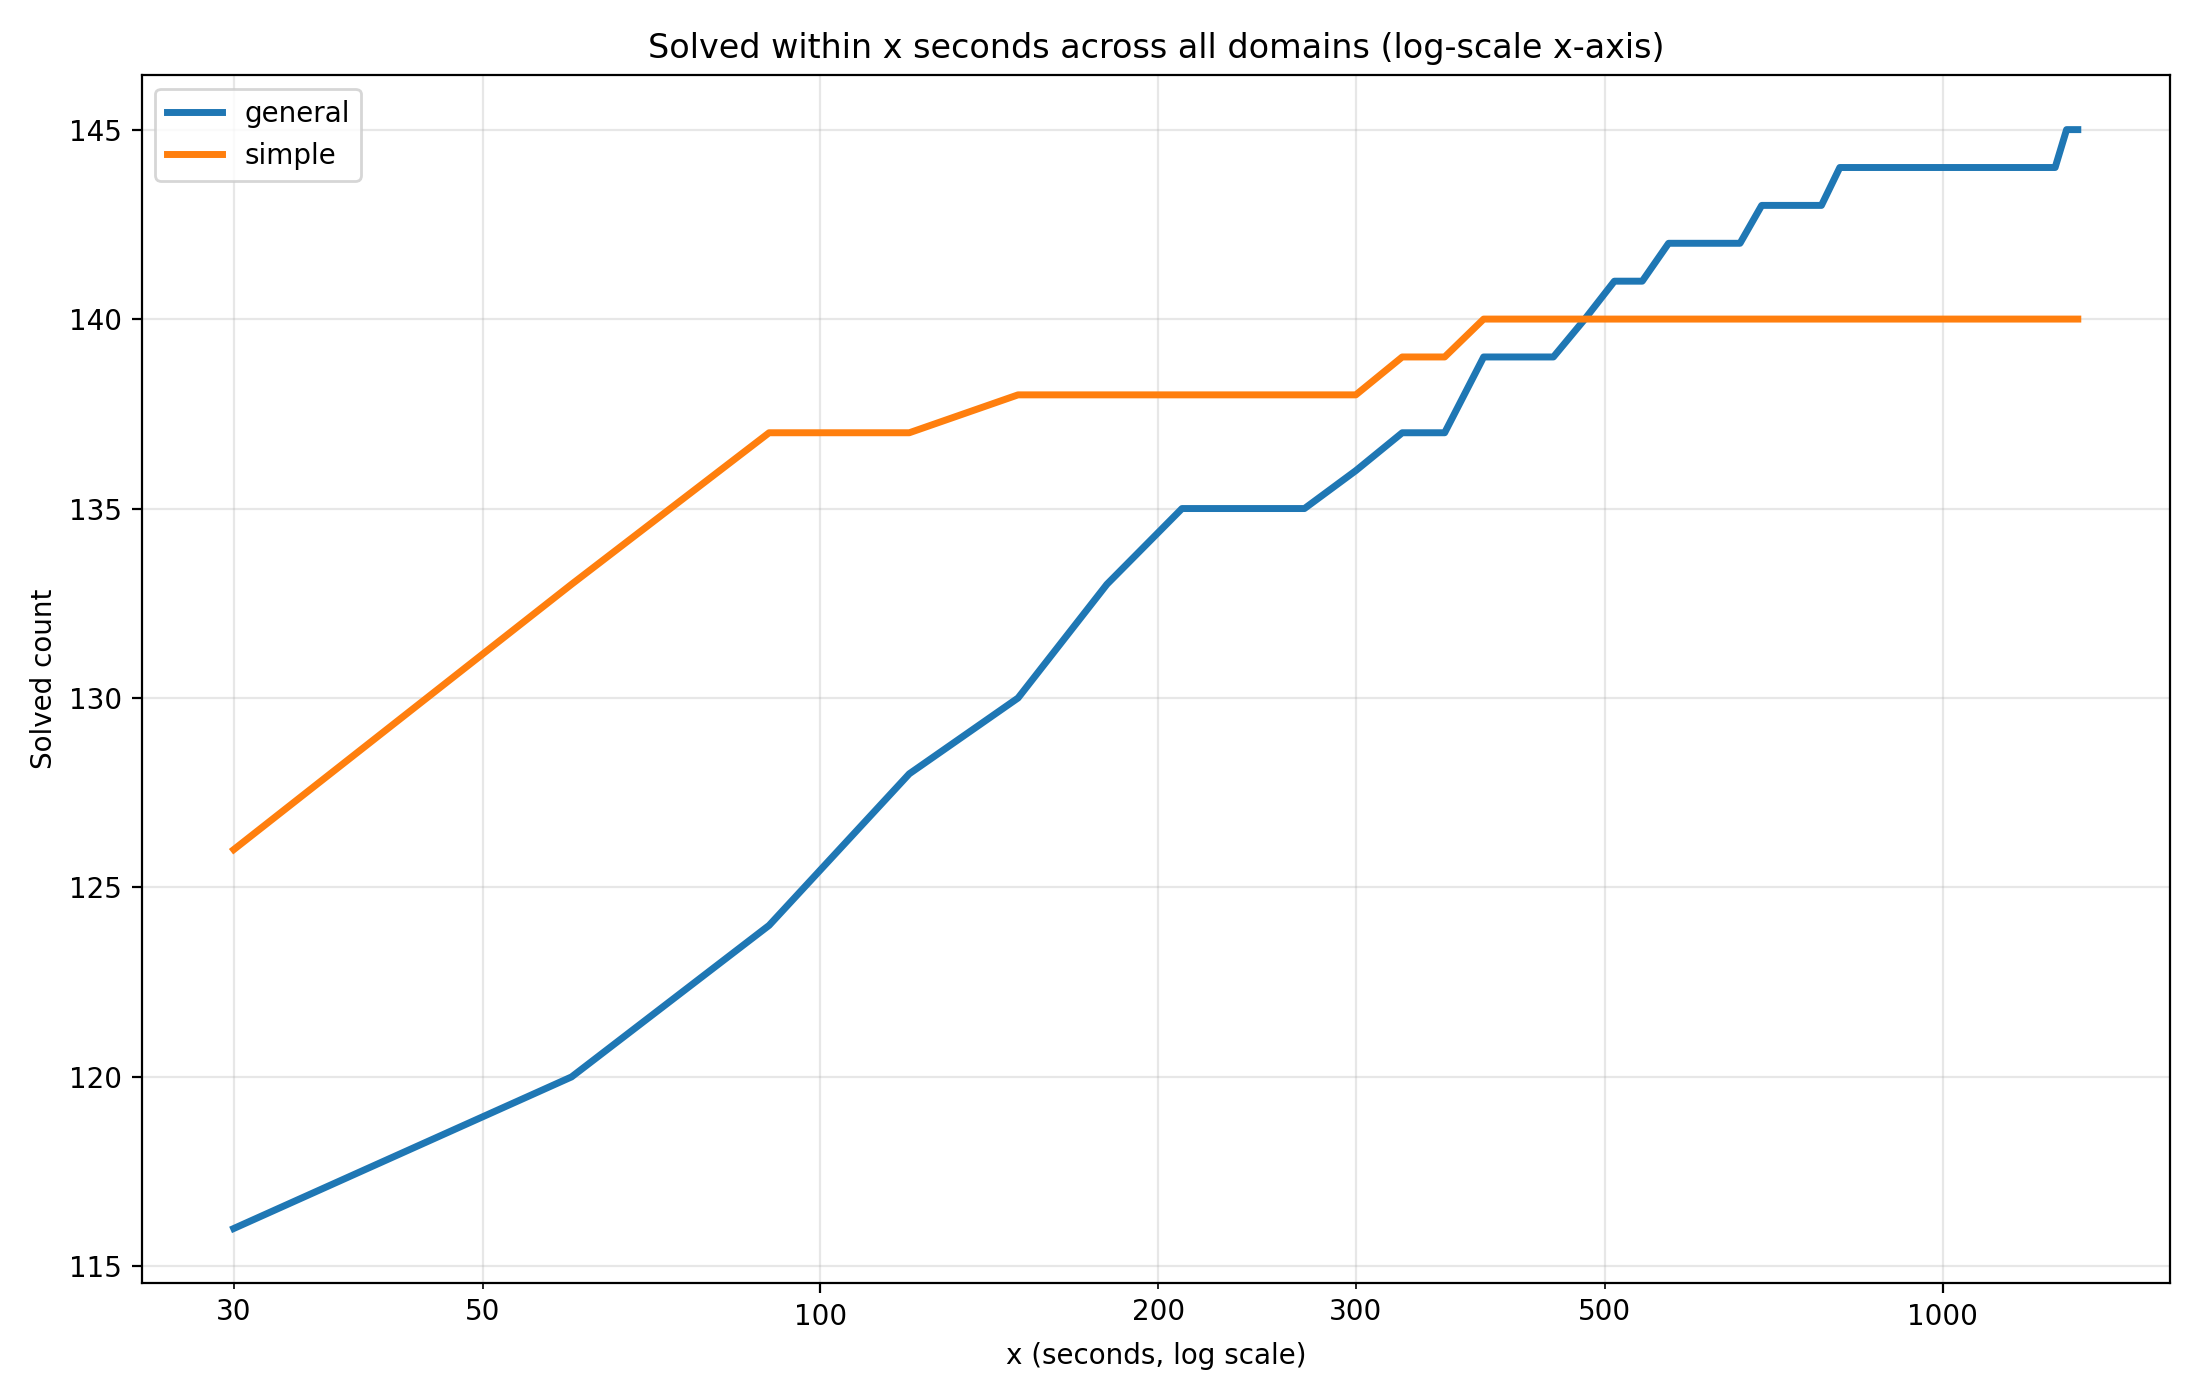
\includegraphics[width=0.82\linewidth]{experimentation/runs/all_domains_tests/analysis/solved_under_time__overall_by_verifier__excluding_numeric_civ_and_blocksworld__log_x.png}
\caption{Cumulative completed verifier/configuration pairs under increasing time thresholds.}
\label{fig:overall-solved}
\end{figure}

To make the split by verifier and social-law setting visible, Figure~\ref{fig:split-solved} reproduces the four solved-under-time plots generated directly from the run logs.

\begin{figure}[t]
\centering
\begin{minipage}{0.48\linewidth}
\centering
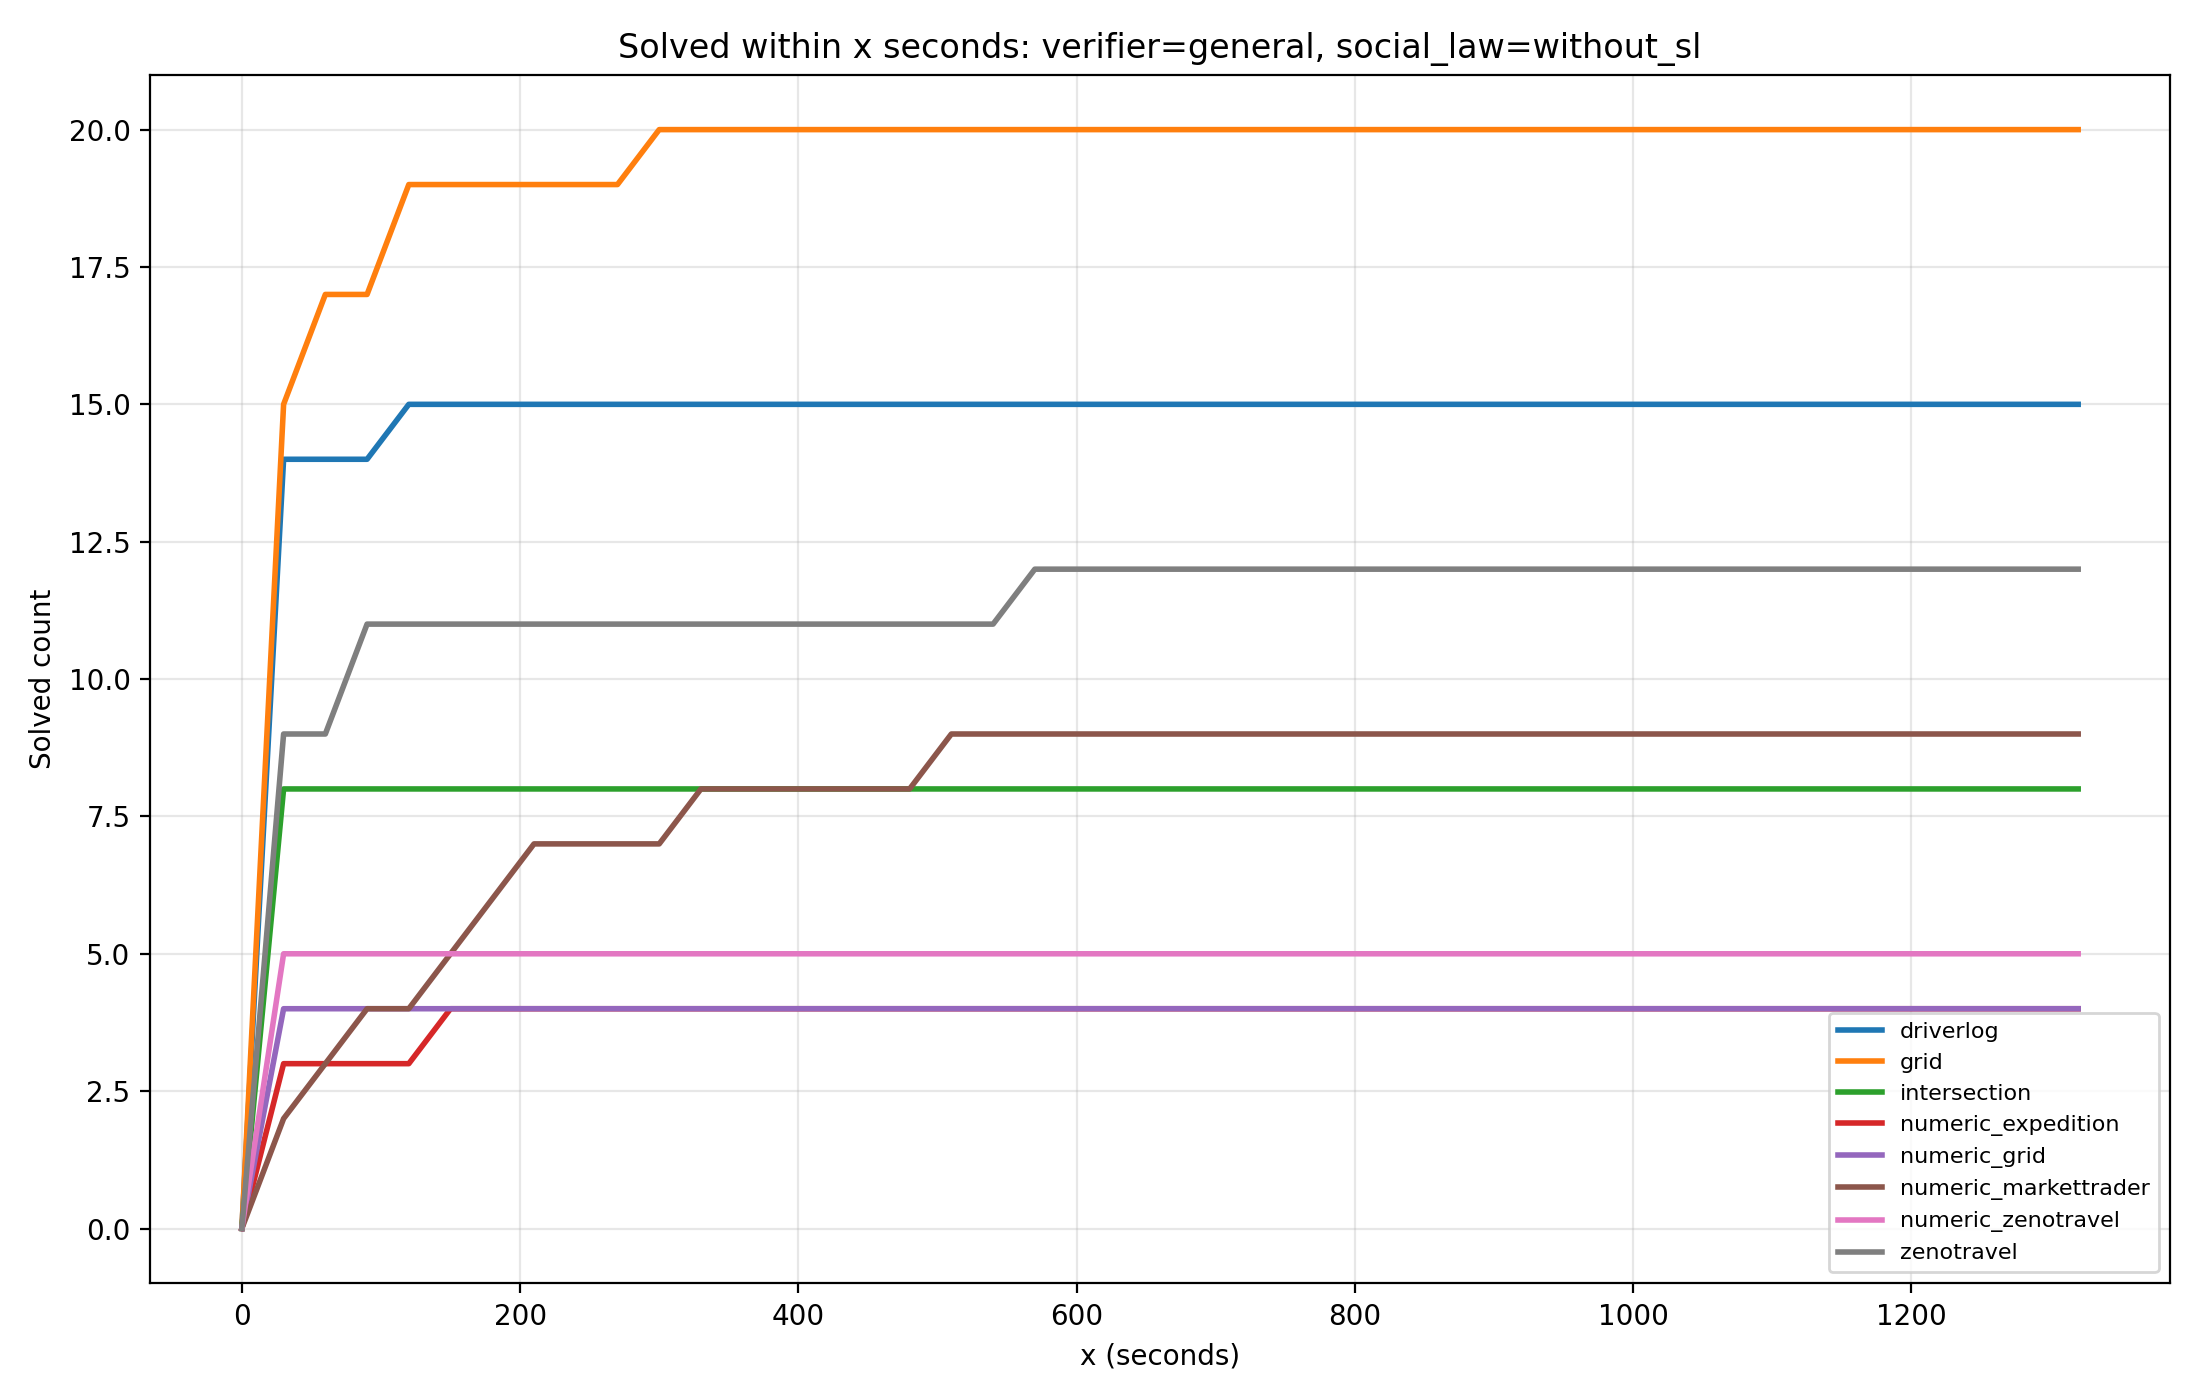
\includegraphics[width=\linewidth]{experimentation/runs/all_domains_tests/analysis/solved_under_time__general__without_sl__excluding_numeric_civ_and_blocksworld.png}
\end{minipage}\hfill
\begin{minipage}{0.48\linewidth}
\centering
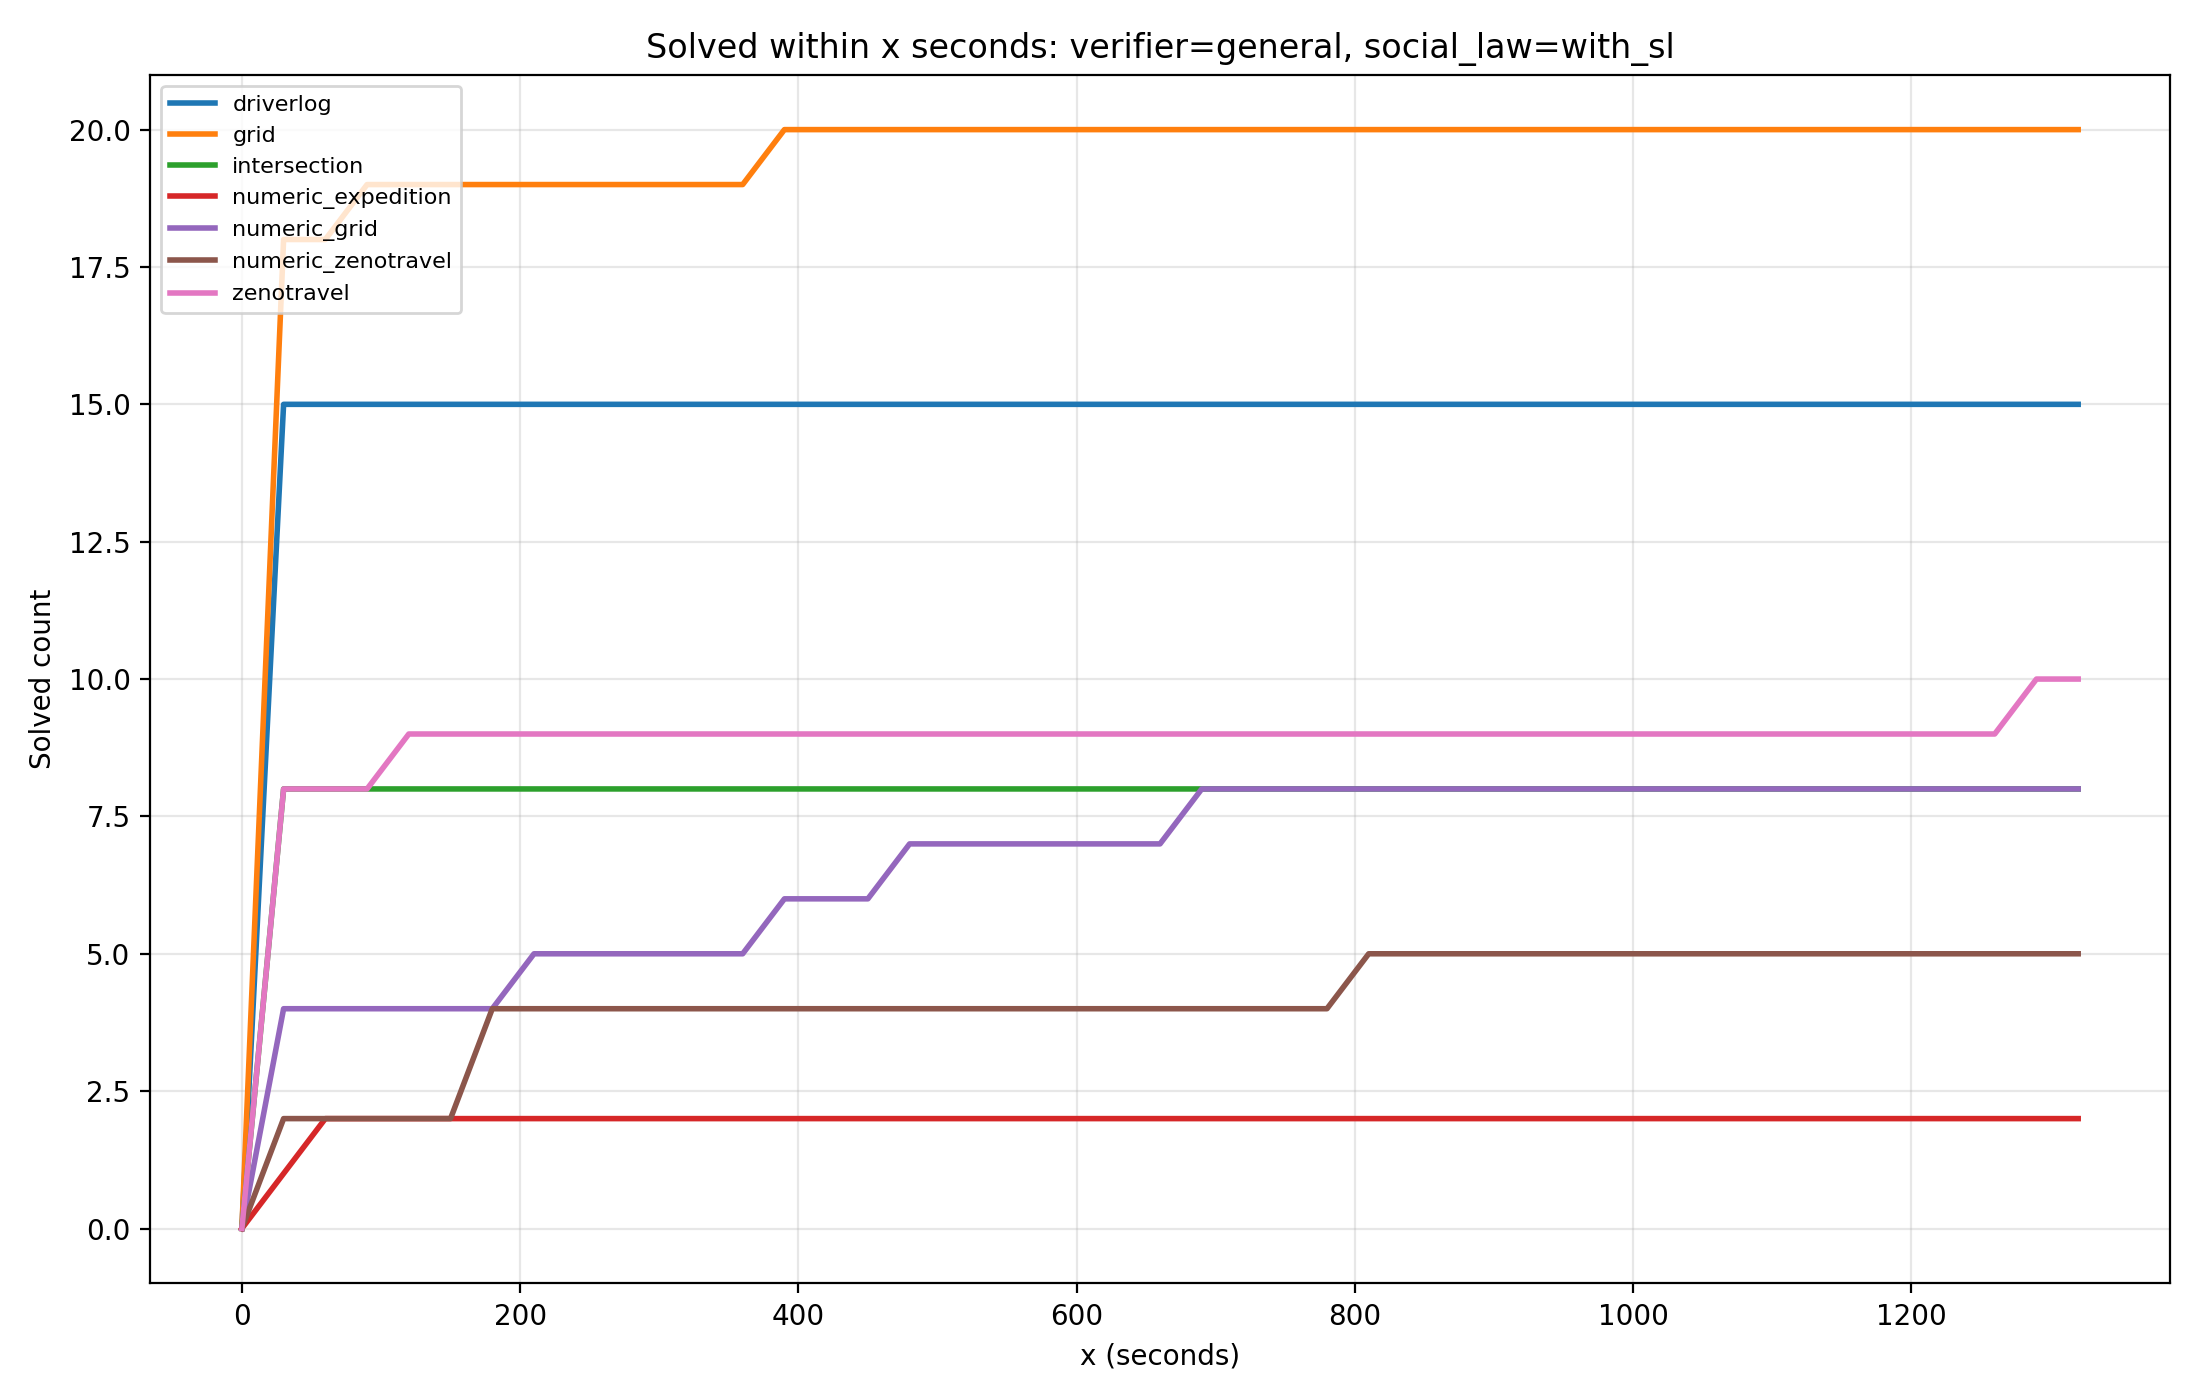
\includegraphics[width=\linewidth]{experimentation/runs/all_domains_tests/analysis/solved_under_time__general__with_sl__excluding_numeric_civ_and_blocksworld.png}
\end{minipage}

\medskip

\begin{minipage}{0.48\linewidth}
\centering
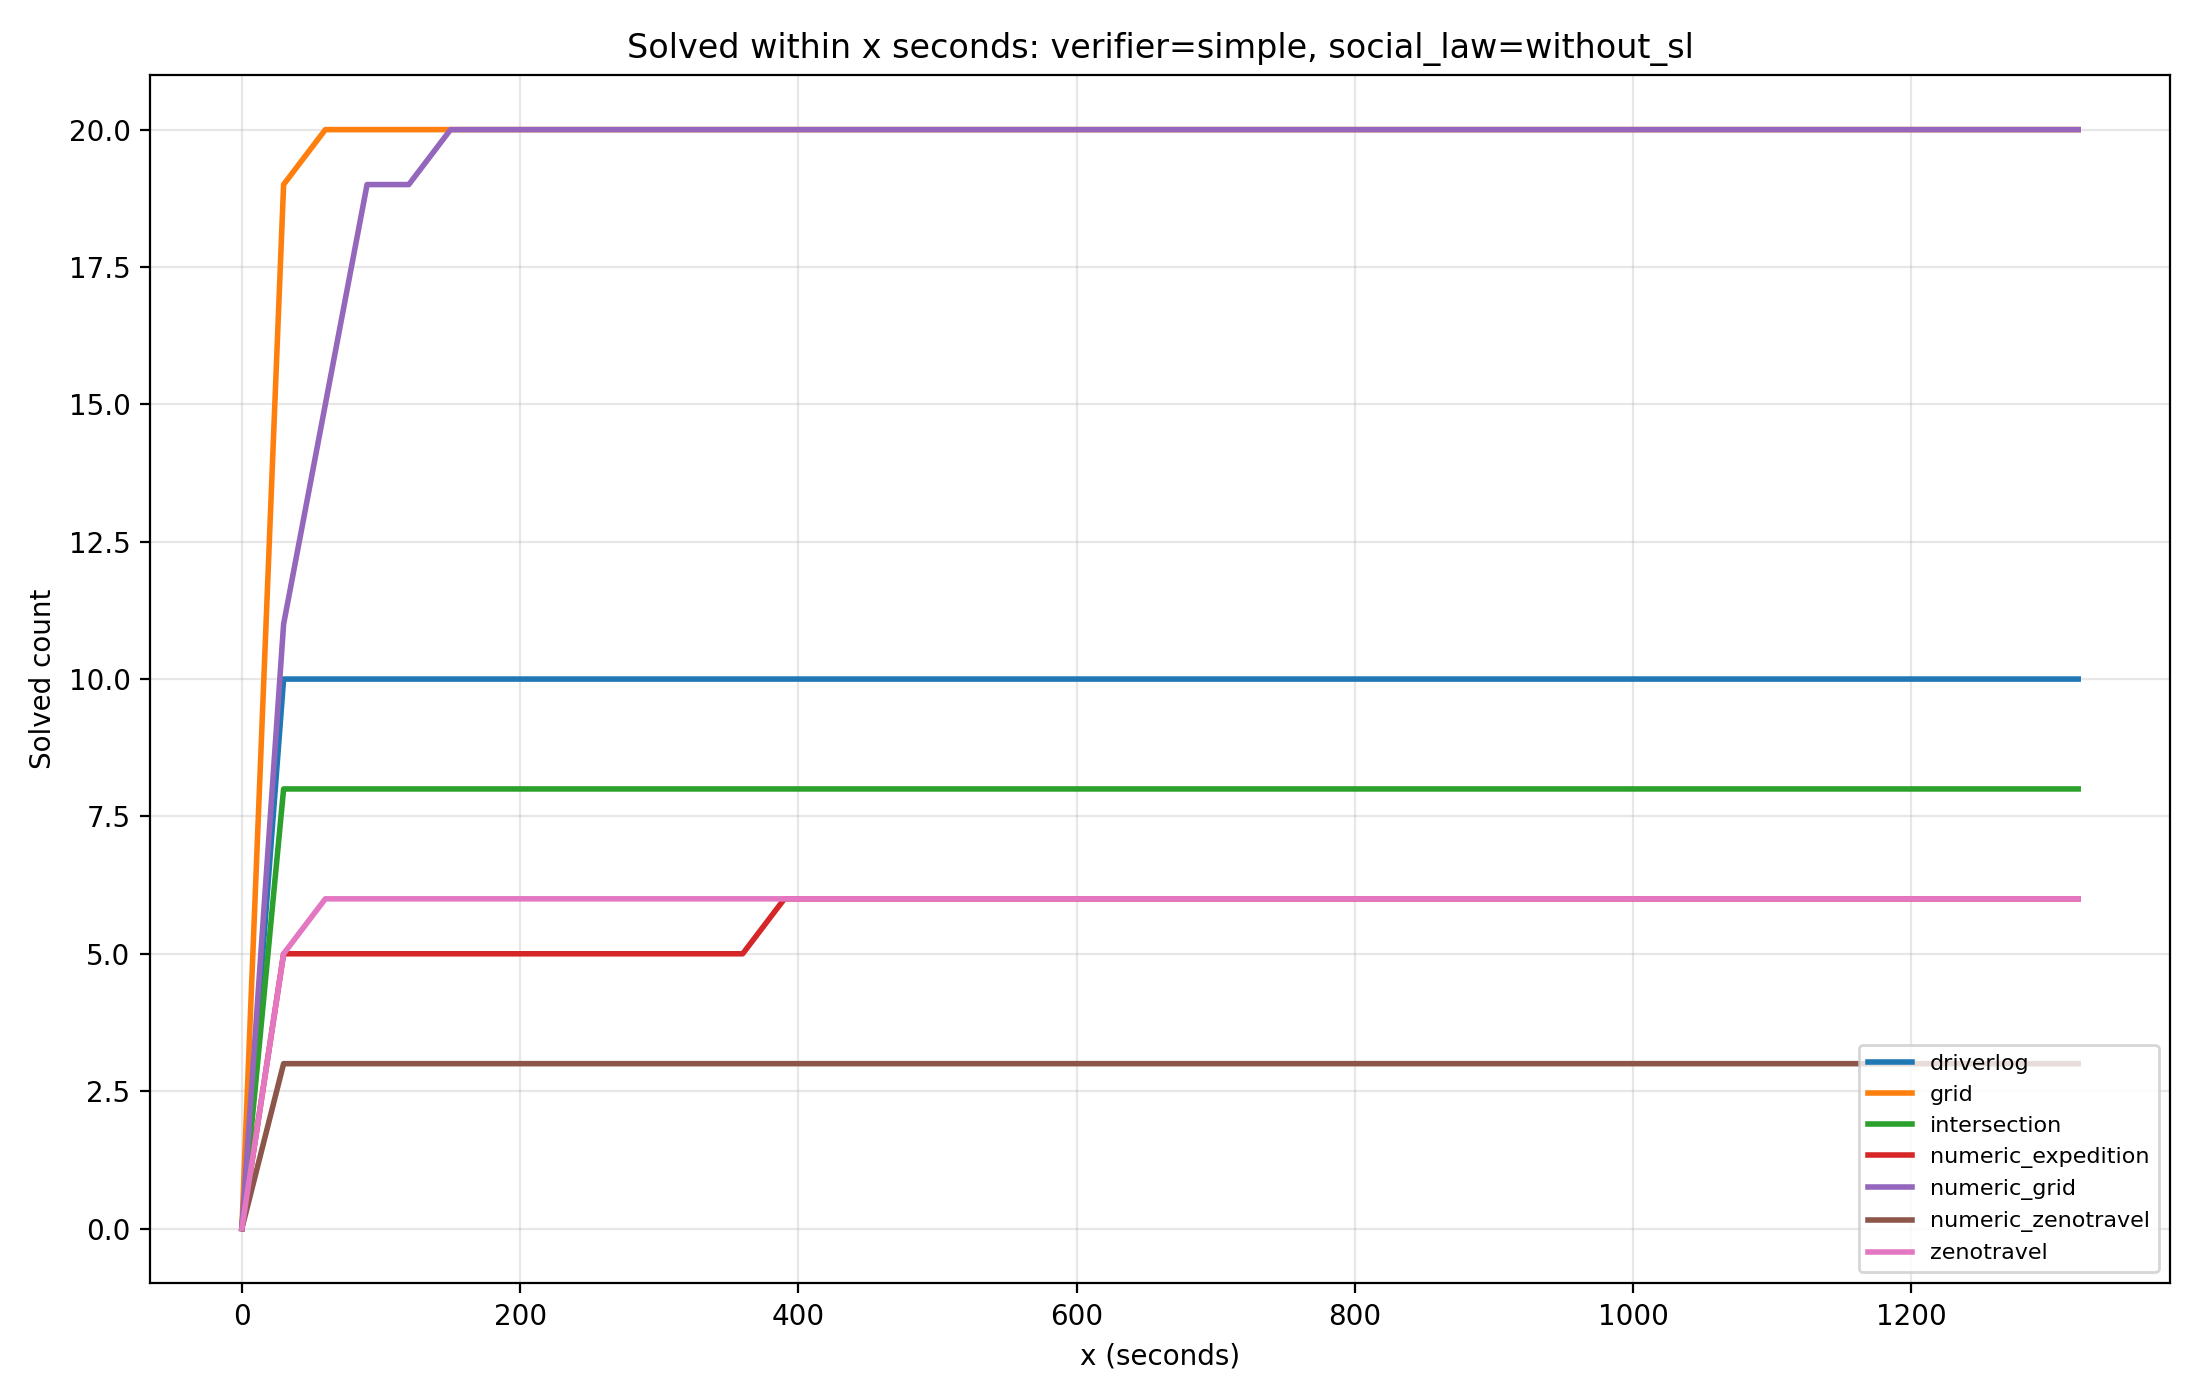
\includegraphics[width=\linewidth]{experimentation/runs/all_domains_tests/analysis/solved_under_time__simple__without_sl__excluding_numeric_civ_and_blocksworld.png}
\end{minipage}\hfill
\begin{minipage}{0.48\linewidth}
\centering
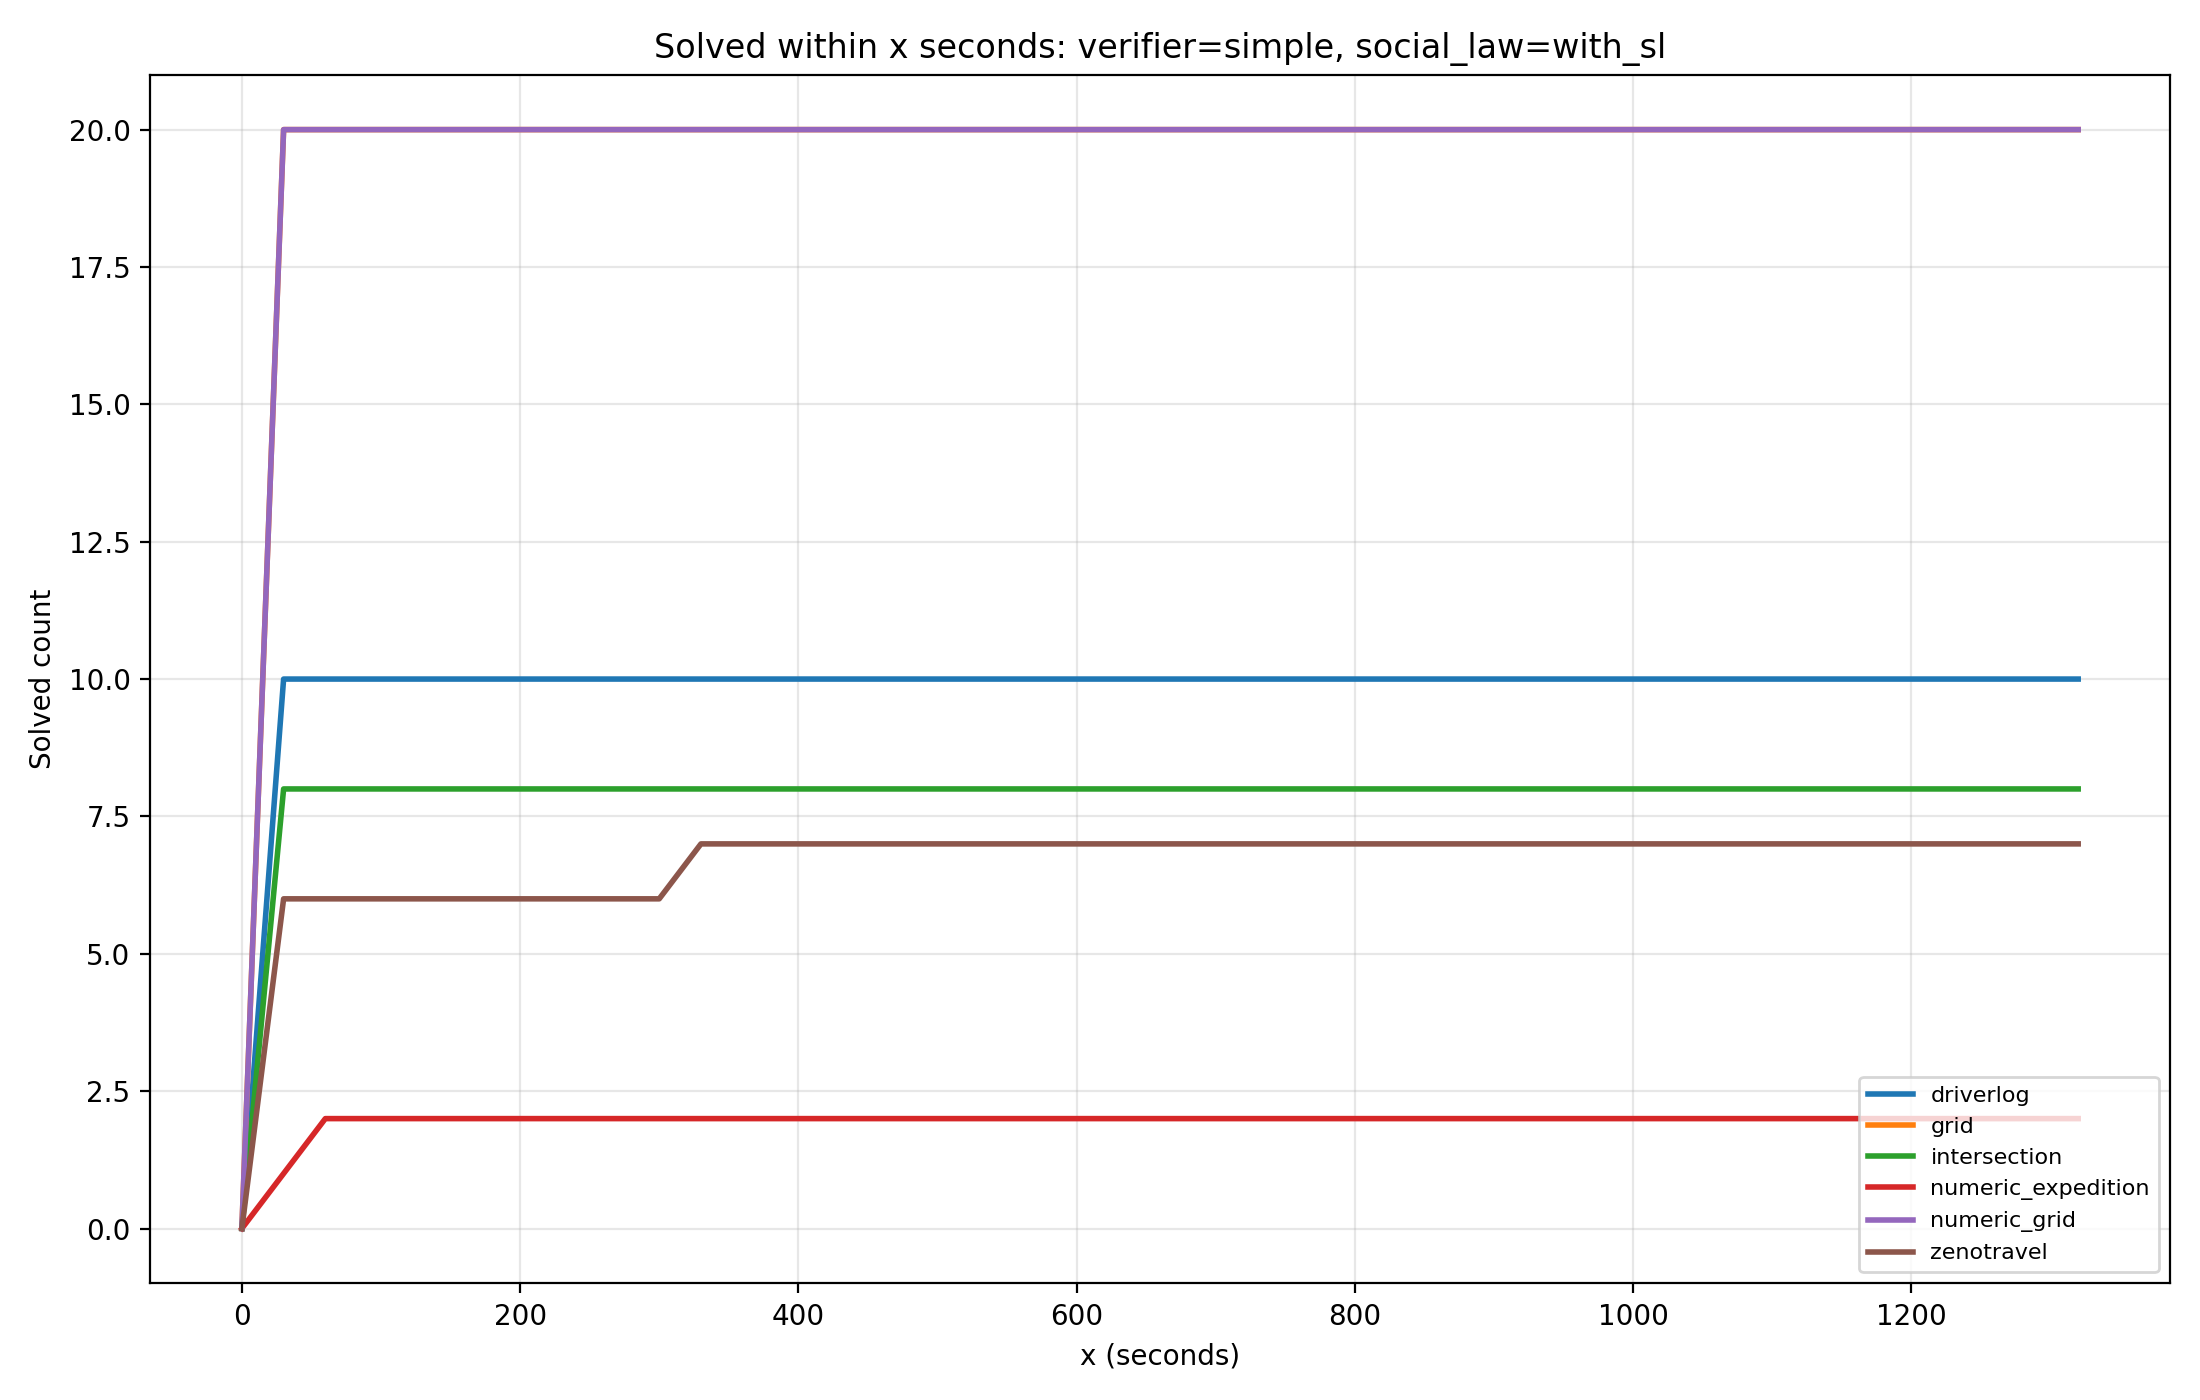
\includegraphics[width=\linewidth]{experimentation/runs/all_domains_tests/analysis/solved_under_time__simple__with_sl__excluding_numeric_civ_and_blocksworld.png}
\end{minipage}
\caption{Solved-under-time curves split by verifier and by whether a social law is enabled. Top row: general verifier. Bottom row: simple verifier. Left: without social law. Right: with social law.}
\label{fig:split-solved}
\end{figure}

\subsection{Discussion}

The run does not support a single global winner; instead it exposes a domain-dependent trade-off between the two implementations.

Across the filtered set of 322 configurations, the general verifier completes 146 cases and the simple verifier completes 141. This does not erase the speed advantage of the simple verifier on easy cases: it still reaches 127 completed pairs within 30 seconds, compared to 117 for the general verifier. But beyond the earliest portion of the curve, the general verifier catches up and ultimately finishes ahead.

\paragraph{Domain behavior is strongly heterogeneous.}
Several domains clearly favor the general verifier: it completes 15 vs.\ 10 instances on both \texttt{driverlog} settings, 12 vs.\ 6 and 10 vs.\ 7 on \texttt{zenotravel}, and it is the only verifier to solve any \texttt{numeric\_markettrader} instances (9 without a social law). In contrast, the simple verifier dominates \texttt{numeric\_grid}, solving all 20 instances both with and without a social law, whereas the general verifier solves only 8 and 4 respectively. Some domains are essentially neutral in this run, notably \texttt{grid} and \texttt{intersection}, where both verifiers have identical completion counts.

% ============================================================
\section{Conclusion}
% ============================================================

We have surveyed three compilation-based approaches to verifying social law robustness in multi-agent planning. The central technical insight shared by all three is the $(n+1)$-copy encoding: maintain one local copy per agent (tracking individual execution) and one global copy (tracking the adversarial joint execution), then search for a configuration that succeeds locally for every agent but fails globally.

The main technical advances across the sequence of works are: (i) the extension from Boolean to numeric state (Nir et al.), which also fixes a deadlock-preservation error in the original; (ii) the generalization to arbitrary instantaneous-action formalisms via explicit stage separation (Tuisov et al.), which subsumes the earlier compilations and opens the door to social laws in richer planning models.

The empirical picture from our completed run is more nuanced than the simplified story often told in the prior papers. Neither verifier dominates overall. The simple verifier has a real speed advantage on easy counterexample-rich cases and performs extremely well on \texttt{numeric\_grid}; the general verifier is much stronger at proving robustness and performs better on several harder domains, including \texttt{driverlog}, \texttt{zenotravel}, and \texttt{numeric\_markettrader}. At the same time, the run reveals concrete engineering issues---especially \texttt{intersection} worker failures and \texttt{numeric\_expedition} internal errors---that should be addressed before treating the present coverage numbers as a definitive comparison.

\bibliographystyle{plain}
\begin{thebibliography}{99}

\bibitem{tennenholtz1989}
M.\ Tennenholtz and Y.\ Moses.
On cooperation in a multi-entity model.
In \emph{IJCAI}, pages 918--923, 1989.

\bibitem{brafman2008}
R.\ I.\ Brafman and C.\ Domshlak.
From one to many: Planning for loosely coupled multi-agent systems.
In \emph{ICAPS}, pages 28--35, 2008.

\bibitem{karpas2017}
E.\ Karpas, A.\ Shleyfman, and M.\ Tennenholtz.
Automated verification of social law robustness in STRIPS.
In \emph{ICAPS}, pages 163--171, 2017.

\bibitem{nir2023}
R.\ Nir, A.\ Shleyfman, and E.\ Karpas.
Automated verification of social laws in numeric settings.
In \emph{AAAI}, pages 12087--12094, 2023.

\bibitem{tuisov2025}
A.\ Tuisov, E.\ Mishlyakov, A.\ Shleyfman, and E.\ Karpas.
Towards a unified view of social laws with instantaneous actions.
In \emph{IJCAI}, 2025.

\bibitem{tuisov2020}
A.\ Tuisov and E.\ Karpas.
Automated verification of social law robustness for reactive agents.
In \emph{ECAI}, volume 325, pages 2386--2393, 2020.

\bibitem{hoffmann2003}
J.\ Hoffmann.
The metric-FF planning system: Translating ``ignoring delete lists'' to numeric state variables.
\emph{JAIR}, 20:291--341, 2003.

\bibitem{helmert2002}
M.\ Helmert.
Decidability and undecidability results for planning with numerical state variables.
In \emph{AIPS}, pages 303--312, 2002.

\bibitem{helmert2006}
M.\ Helmert.
New complexity results for classical planning benchmarks.
In \emph{ICAPS}, pages 52--61, 2006.

\bibitem{scala2020}
E.\ Scala et al.
Subgoaling techniques for satisficing and optimal numeric planning.
\emph{JAIR}, 68:691--752, 2020.

\bibitem{stolba2015}
M.\ Stolba, A.\ Komenda, and D.\ L.\ Kovacs.
Competition of distributed and multiagent planners (CoDMAP).
\emph{http://agents.fel.cvut.cz/codmap/}, 2015.

\bibitem{upf2025}
Unified Planning Framework.
Unified planning: Modeling, manipulating and solving AI planning problems in Python.
\emph{SoftwareX}, 29:102012, 2025.

\end{thebibliography}

\end{document}
